%\thispagestyle{myheadings}
\section{Invited Talk: Nando de Freitas}
\index{de Freitas, Nando}

\begin{center}
\begin{Large}
{\bfseries\Large Physical simulation, learning and language}
\vspace{1em}\par
\end{Large}

\daydateyear, 9:00--10:10am \vspace{1em}\\
\PlenaryLoc \\
\vspace{1em}\par
%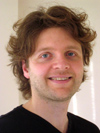
\includegraphics[height=100px]{content/tuesday/popovic-headshot.jpg}
\end{center}

\noindent
{\bfseries Abstract:} Simulated physical environments, with common physical laws, objects and agents with bodies, provide us with consistency to facilitate transfer and continual learning. In such environments, research topics such as learning to experiment, learning to learn and emergent communication can be easily explored. Given the relevance of these topics to language, it is natural to ask ourselves whether research in language would benefit from the development of such environments, and whether language can contribute toward improving such environments and agents within them. This talk will provide an overview of some of these environments, discuss learning to learn and its potential relevance to language, and present some deep reinforcement learning agents that capitalize on formal language instructions to develop disentangled interpretable representations that allow them to generalize to a wide variety of zero-shot semantic tasks. The talk will pose more questions than answers in the hope of stimulating discussion. 

\vspace{3em}\par 

\vfill
\noindent

{\bfseries Biography:} 
I was born in Zimbabwe, with malaria. I was a refugee from the war in Mocambique and thanks to my parents getting in debt to buy me a passport from a corrupt official, I grew up in Portugal without water and electricity, before the EU got there, and without my parents who were busy making money to pay their debt. At 8, I joined my parents in Venezuela and began school in the hood; see City of God. I moved to South Africa after high-school and sold beer illegally in black-townships for a living until 1991. Apartheid was the worst thing I ever experienced. I did my BSc in electrical engineering and MSc in control at the University of the Witwatersrand, where I strived to be the best student to prove to racists that anyone can do it. I did my PhD on Bayesian methods for neural networks at Trinity College, Cambridge University. I did a postdoc in Artificial Intelligence at UC Berkeley. I became a Full Professor at the University of British Columbia, before joining the University of Oxford in 2013. I quit Oxford in 2017 to join DeepMind full-time, where I lead the Machine Learning team. I aim to solve intelligence so that future generations have a better life. I have been a Senior Fellow of the Canadian Institute for Advanced Research for a long time. Some of my recent awards, mostly thanks to my collaborators, include: Best Paper Award at the International Conference on Machine Learning (2016), Best Paper Award at the International Conference on Learning Representations (2016), Winner of round 5 of the Yelp Dataset Challenge (2015), Distinguished Paper Award at the International Joint Conference on Artificial Intelligence (2013), Charles A. McDowell Award for Excellence in Research (2012), and Mathematics of Information Technology and Complex Systems Young Researcher Award (2010). 

\newpage
